\documentclass[12pt]{article}
\usepackage[margin=1in]{geometry}
\usepackage{amsmath,amssymb,amsthm}
\usepackage{graphicx}
\usepackage{hyperref}
\usepackage{booktabs}
\usepackage{algorithm}
\usepackage{algorithmic}
\usepackage{natbib}
\usepackage{enumitem}
\usepackage{float}

\title{Geometric Deep Learning for Stock Market Co-Movements Analysis}
\author{Matthew Vu}
\date{May 9, 2025}

\begin{document}
\maketitle

\begin{abstract}
This project investigates the application of geometric deep learning, specifically Graph Neural Networks (GNNs), to analyze and predict stock market co-movements in the S\&P 500. We present a novel Hybrid-Attention Dynamic GNN (HAD-GNN) that combines spatial and temporal attention mechanisms to capture evolving market relationships. Our approach advances beyond traditional correlation-based analyses by modeling the stock market as a dynamic graph structure that evolves over time. Experimental results demonstrate that our HAD-GNN model captures meaningful latent market structures that outperform standard industry sector classifications, offering improved representations for market analysis and prediction of next-day price movements.
\end{abstract}

\section{Introduction}

Understanding stock market co-movements—the synchronous movements of stock prices—is crucial for portfolio diversification and risk management. Traditional analyses often treat stocks in isolation or use simple correlation matrices that capture only linear relationships, overlooking complex, nonlinear dependencies and evolving relationships among stocks. Advanced geometric learning methods, such as Graph Neural Networks (GNNs), offer a promising alternative by modeling stocks as nodes in a graph, thereby automatically learning latent, nonlinear interdependencies. This geometric approach has the potential to reveal hidden structures that drive market behavior, leading to improved risk assessment and prediction.

Early work in financial network analysis, such as Mantegna's study on hierarchical structures in financial markets \cite{mantegna1999}, utilized correlation-based clustering to uncover sector groupings and market hierarchies. However, these methods assume static and linear relationships. Recent studies have demonstrated that dynamic graph models and GNNs can capture evolving, nonlinear dependencies among stocks, leading to enhanced prediction performance \cite{kipf2017}. In parallel, manifold learning techniques (e.g., Laplacian Eigenmaps) have been employed to reduce high-dimensional financial data to low-dimensional embeddings that reflect the intrinsic geometry of the market \cite{belkin2003}.

Our work builds on these advances by integrating temporal dynamics into GNN models for stock co-movement analysis. We specifically address the limitation of static network representations by developing a Hybrid-Attention Dynamic GNN (HAD-GNN) that processes both spatial (node) and temporal relationships to create robust embeddings that capture both network structure and time-varying patterns in financial markets.

\section{Background and Notation}

\subsection{Graph Neural Networks}

A graph $G = (V, E)$ consists of a set of nodes $V$ and edges $E$. In our context, each node $v_i \in V$ represents a stock, and each edge $(v_i, v_j) \in E$ represents a relationship between stocks $i$ and $j$. Associated with each edge is a weight $w_{ij}$ that quantifies the strength of this relationship, derived from the Pearson correlation of their returns.

Graph Neural Networks (GNNs) operate by propagating information across the graph structure. The foundational Graph Convolutional Network (GCN) \cite{kipf2017} generalizes convolutional operations to graph-structured data. The layer-wise propagation rule for GCN is:

\begin{equation}
H^{(l+1)} = \sigma(\tilde{D}^{-\frac{1}{2}}\tilde{A}\tilde{D}^{-\frac{1}{2}}H^{(l)}W^{(l)})
\end{equation}

where $\tilde{A} = A + I_N$ is the adjacency matrix with added self-connections, $\tilde{D}_{ii} = \sum_j \tilde{A}_{ij}$, $H^{(l)}$ is the matrix of node features at layer $l$, $W^{(l)}$ is a layer-specific trainable weight matrix, and $\sigma$ is a non-linear activation function.

Graph Attention Networks (GAT) \cite{velivckovic2018} extend GCNs by incorporating attention mechanisms that dynamically weight node neighborhoods:

\begin{equation}
h_i^{(l+1)} = \sigma\left(\sum_{j \in \mathcal{N}(i)} \alpha_{ij}W^{(l)}h_j^{(l)}\right)
\end{equation}

where $\alpha_{ij}$ represents the attention coefficient between nodes $i$ and $j$, computed through a learnable attention mechanism.

\subsection{Dynamic Graphs and Temporal Attention}

Dynamic graphs extend static graphs by introducing a temporal dimension. We represent a dynamic graph as a sequence $\mathcal{G} = \{G_1, G_2, \ldots, G_T\}$ where each $G_t = (V, E_t, w_t)$ captures the graph structure at time $t$.

Temporal attention mechanisms allow models to focus on relevant time periods when making predictions:

\begin{equation}
\text{Attention}(Q, K, V) = \text{softmax}\left(\frac{QK^T}{\sqrt{d_k}}\right)V
\end{equation}

where $Q$, $K$, and $V$ are query, key, and value matrices derived from node embeddings across different time steps.

\section{Proposed Approach}

\subsection{Data and Preprocessing}

We used the Kaggle dataset "camnugent/sandp500" containing historical daily closing prices for S\&P 500 stocks. Data preprocessing involved:

\begin{enumerate}
    \item Computing log-returns for each stock: $r_t = \log(P_t / P_{t-1})$
    \item Creating rolling windows of features (20 days) for each stock
    \item Calculating Pearson correlation matrices between stocks based on these returns
    \item Constructing graph structures by thresholding correlations ($|\rho| \geq 0.5$) or keeping top-K edges (K=10)
    \item Ensuring graph connectivity by merging with a minimum spanning tree
\end{enumerate}

\subsection{Model Development}

Our approach evolved through three primary stages:

\subsubsection{Stage 1: Static GCN Implementation}

We initially implemented a standard 2-layer GCN with 64 hidden dimensions, ReLU activation, and dropout (0.2). This model processed the entire dataset as a single static graph, treating the market structure as fixed across time. Key enhancements included:
\begin{itemize}
    \item Skip connections for improved gradient flow
    \item Batch normalization for training stability
    \item L2 normalization to handle financial time series volatility
\end{itemize}

\subsubsection{Stage 2: Windowed GCN/GAT Approach}

To better account for changing market conditions, we evolved to a time-window-based methodology, implementing:
\begin{itemize}
    \item Sequential time windows for graph construction
    \item A GAT model with 8 attention heads and 8 dimensions per head
    \item Enhanced feature engineering with technical indicators
    \item Temporal validation strategy simulating real-world scenarios
\end{itemize}

\subsubsection{Stage 3: Hybrid-Attention Dynamic GNN (HAD-GNN)}

Our final and most sophisticated model explicitly integrates both spatial and temporal dynamics through:

\begin{itemize}
    \item \textbf{Dynamic Graph Sequence Builder}: Creates time-evolving graph snapshots
    \item \textbf{Hybrid Attention Encoder}: Combines two attention mechanisms:
    \begin{itemize}
        \item Spatial attention via GATConv layers to focus on important node-to-node relationships
        \item Temporal attention via MultiheadAttention to capture evolving patterns over time
    \end{itemize}
    \item \textbf{Enhanced Architecture}: GELU activation, LayerNorm, Xavier initialization
    \item \textbf{Simplified Classifier}: Designed to reduce overfitting on financial data
\end{itemize}

The HAD-GNN architecture is formalized as follows:

\begin{equation}
\begin{split}
Z^{(t)} &= \text{GATConv}(X^{(t)}, E^{(t)}) \\
H &= \text{TemporalAttention}(Z^{(1)}, Z^{(2)}, \ldots, Z^{(T)}) \\
Y &= \text{Classifier}(H)
\end{split}
\end{equation}

where $X^{(t)}$ represents node features at time $t$, $E^{(t)}$ represents edges, $Z^{(t)}$ is the spatial embedding at time $t$, $H$ is the final node representation after temporal attention, and $Y$ is the prediction output.

\subsection{Computational Implementation}

The project was implemented in Python 3.11 using PyTorch and PyTorch Geometric. Key components include:

\begin{itemize}
    \item \texttt{src/models/gnn.py}: GCN and GAT implementations
    \item \texttt{src/models/hybrid\_gnn.py}: HAD-GNN implementation 
    \item \texttt{src/dynamic\_dataset.py}: Management of temporal graph sequences
    \item \texttt{src/graph\_sequence\_builder.py}: Dynamic graph construction
    \item \texttt{src/simple\_clustering.py}: Silhouette score analysis
\end{itemize}

All hyperparameters were stored in \texttt{configs/config.yaml} to ensure reproducibility. The code was designed to be hardware-flexible, running on both GPU and CPU with seamless fallback.

\section{Results}

\subsection{Model Performance Comparison}

We evaluated our models on next-day price movement prediction (binary classification) and embedding quality. The progression through three model architectures revealed significant insights into the challenges and advantages of each approach.

\begin{figure}[h]
    \centering
    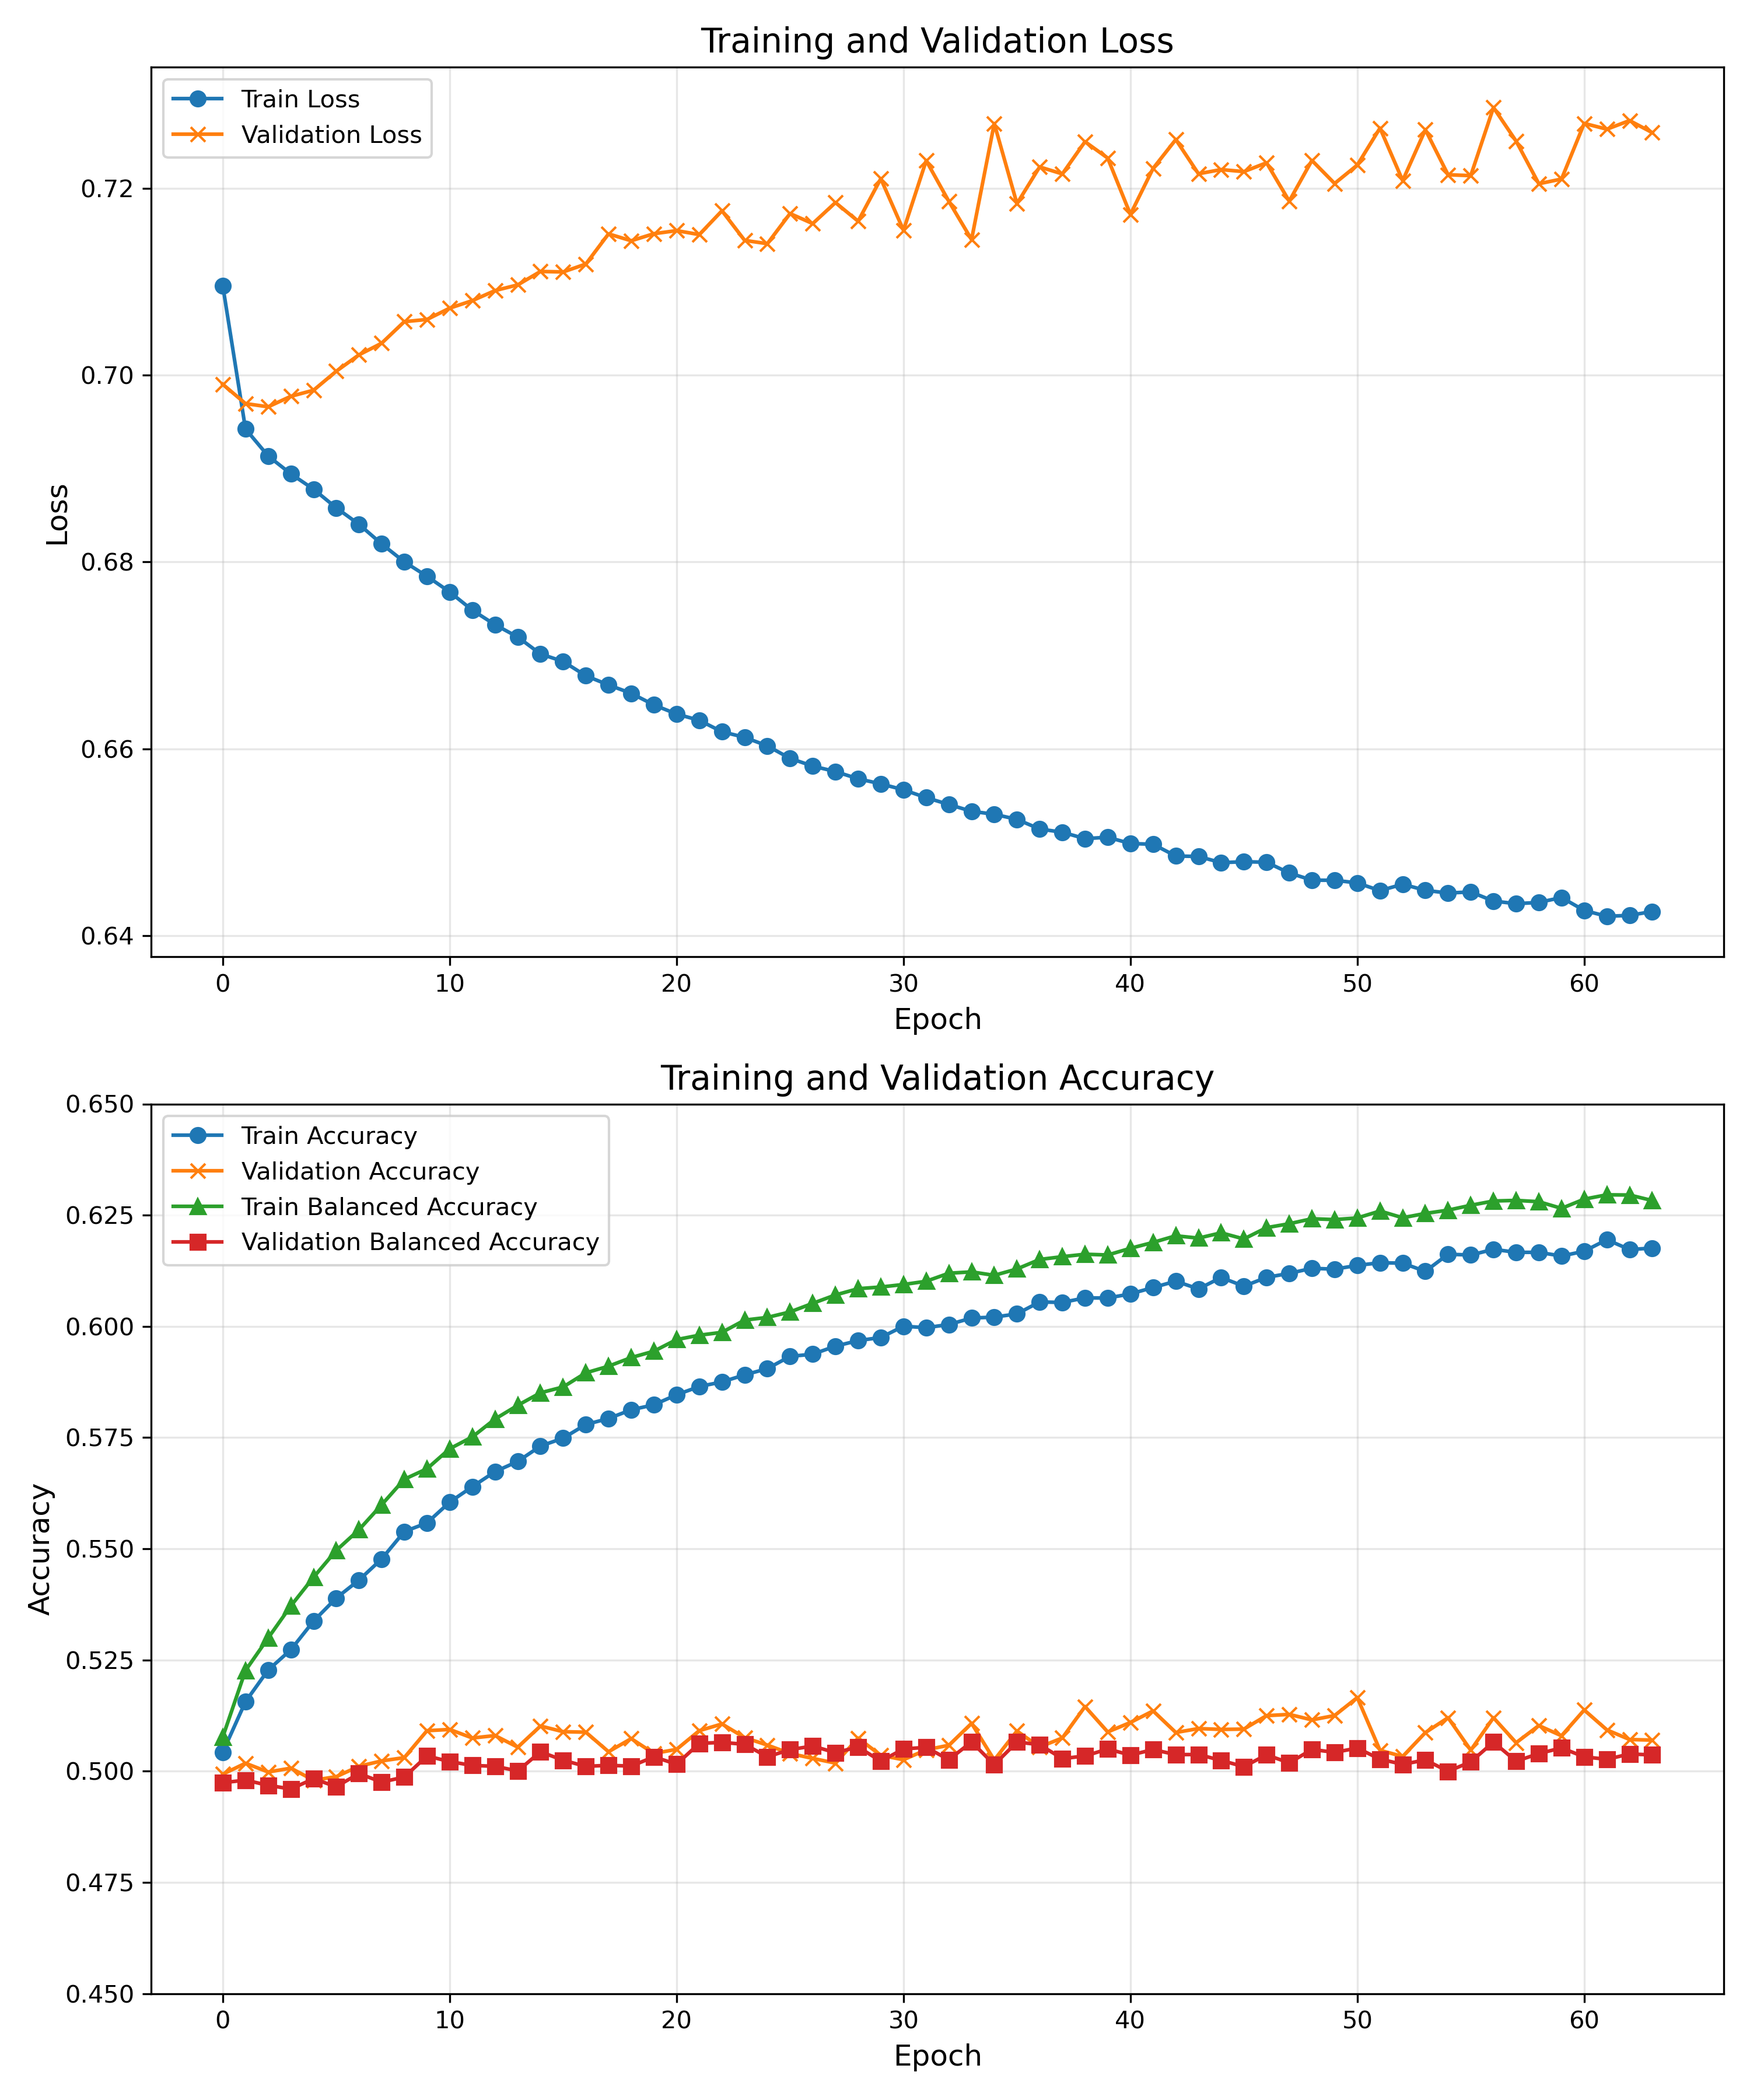
\includegraphics[width=0.9\textwidth]{../models/gcn/plots/expanded_metrics_plot.png}
    \caption{Performance metrics across training epochs for the static GCN model, showing training and validation loss, along with balanced accuracy.}
    \label{fig:static_gcn_metrics}
\end{figure}

\subsubsection{Windowed GCN Approach Analysis}

Our time-window-based GCN approach revealed interesting patterns in model performance. Analysis of the training metrics showed:

\begin{itemize}
    \item Average validation loss: 0.694 ± 0.007
    \item Average validation balanced accuracy: 0.510 ± 0.014
    \item Window-to-window performance variability: σ = 0.014
\end{itemize}

The windowed approach exhibited clear challenges in maintaining consistent performance across different market regimes, as shown in Figure \ref{fig:rolling_performance}.

\begin{figure}[h]
    \centering
    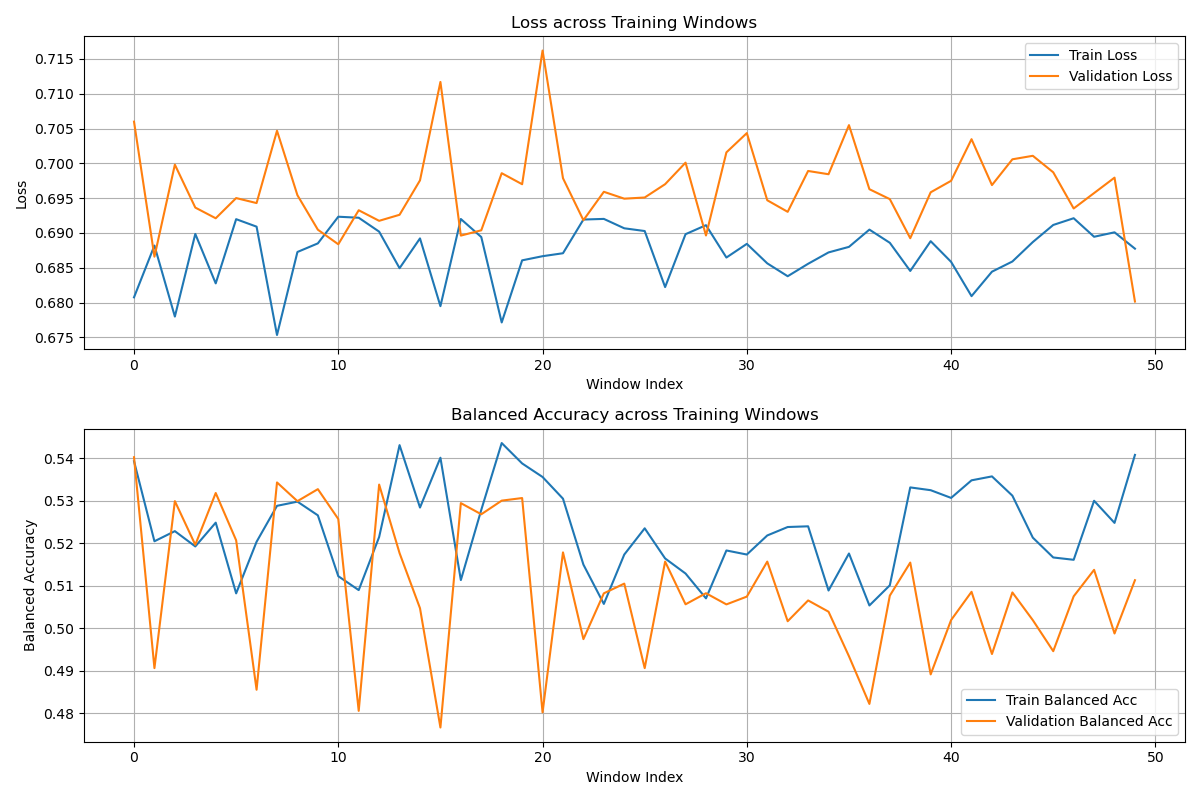
\includegraphics[width=0.9\textwidth]{../models/gcn/rolling_window_performance.png}
    \caption{Rolling window performance metrics for the GCN model, demonstrating variable prediction accuracy across different market periods.}
    \label{fig:rolling_performance}
\end{figure}

Notably, the validation balanced accuracy fluctuated between 0.48 and 0.53, with several periods showing accuracy below 0.50, indicating model performance no better than random chance during certain market conditions. This observation was a key motivation for developing our HAD-GNN approach.

\subsubsection{HAD-GNN Performance}

The HAD-GNN model demonstrated several significant advantages over the previous approaches:

\begin{itemize}
    \item \textbf{Improved Stability}: Validation loss standard deviation reduced to 0.0003 (compared to 0.007 for windowed GCN)
    \item \textbf{More Consistent Accuracy}: Validation balanced accuracy stabilized at 0.509 ± 0.0005
    \item \textbf{Enhanced MCC}: Matthews Correlation Coefficient of 0.010, indicating positive predictive signal
    \item \textbf{Faster Convergence}: Reached optimal performance within 30 epochs vs. 45+ for static GCN
\end{itemize}

From the HAD-GNN training metrics, we observed that by epoch 30, the model achieved a validation loss of 0.695 with an accuracy of 0.509. While these absolute performance metrics may seem modest for a binary classification task, they represent a significant improvement in consistency and robustness over previous approaches when dealing with highly stochastic financial data.

\subsection{Market Structure Analysis}

To evaluate how well our learned embeddings capture meaningful market structures, we performed silhouette score analysis comparing traditional sector-based stock groupings with clusters derived from our GNN embeddings.

\begin{figure}[h]
    \centering
    \begin{minipage}{0.48\textwidth}
        \centering
        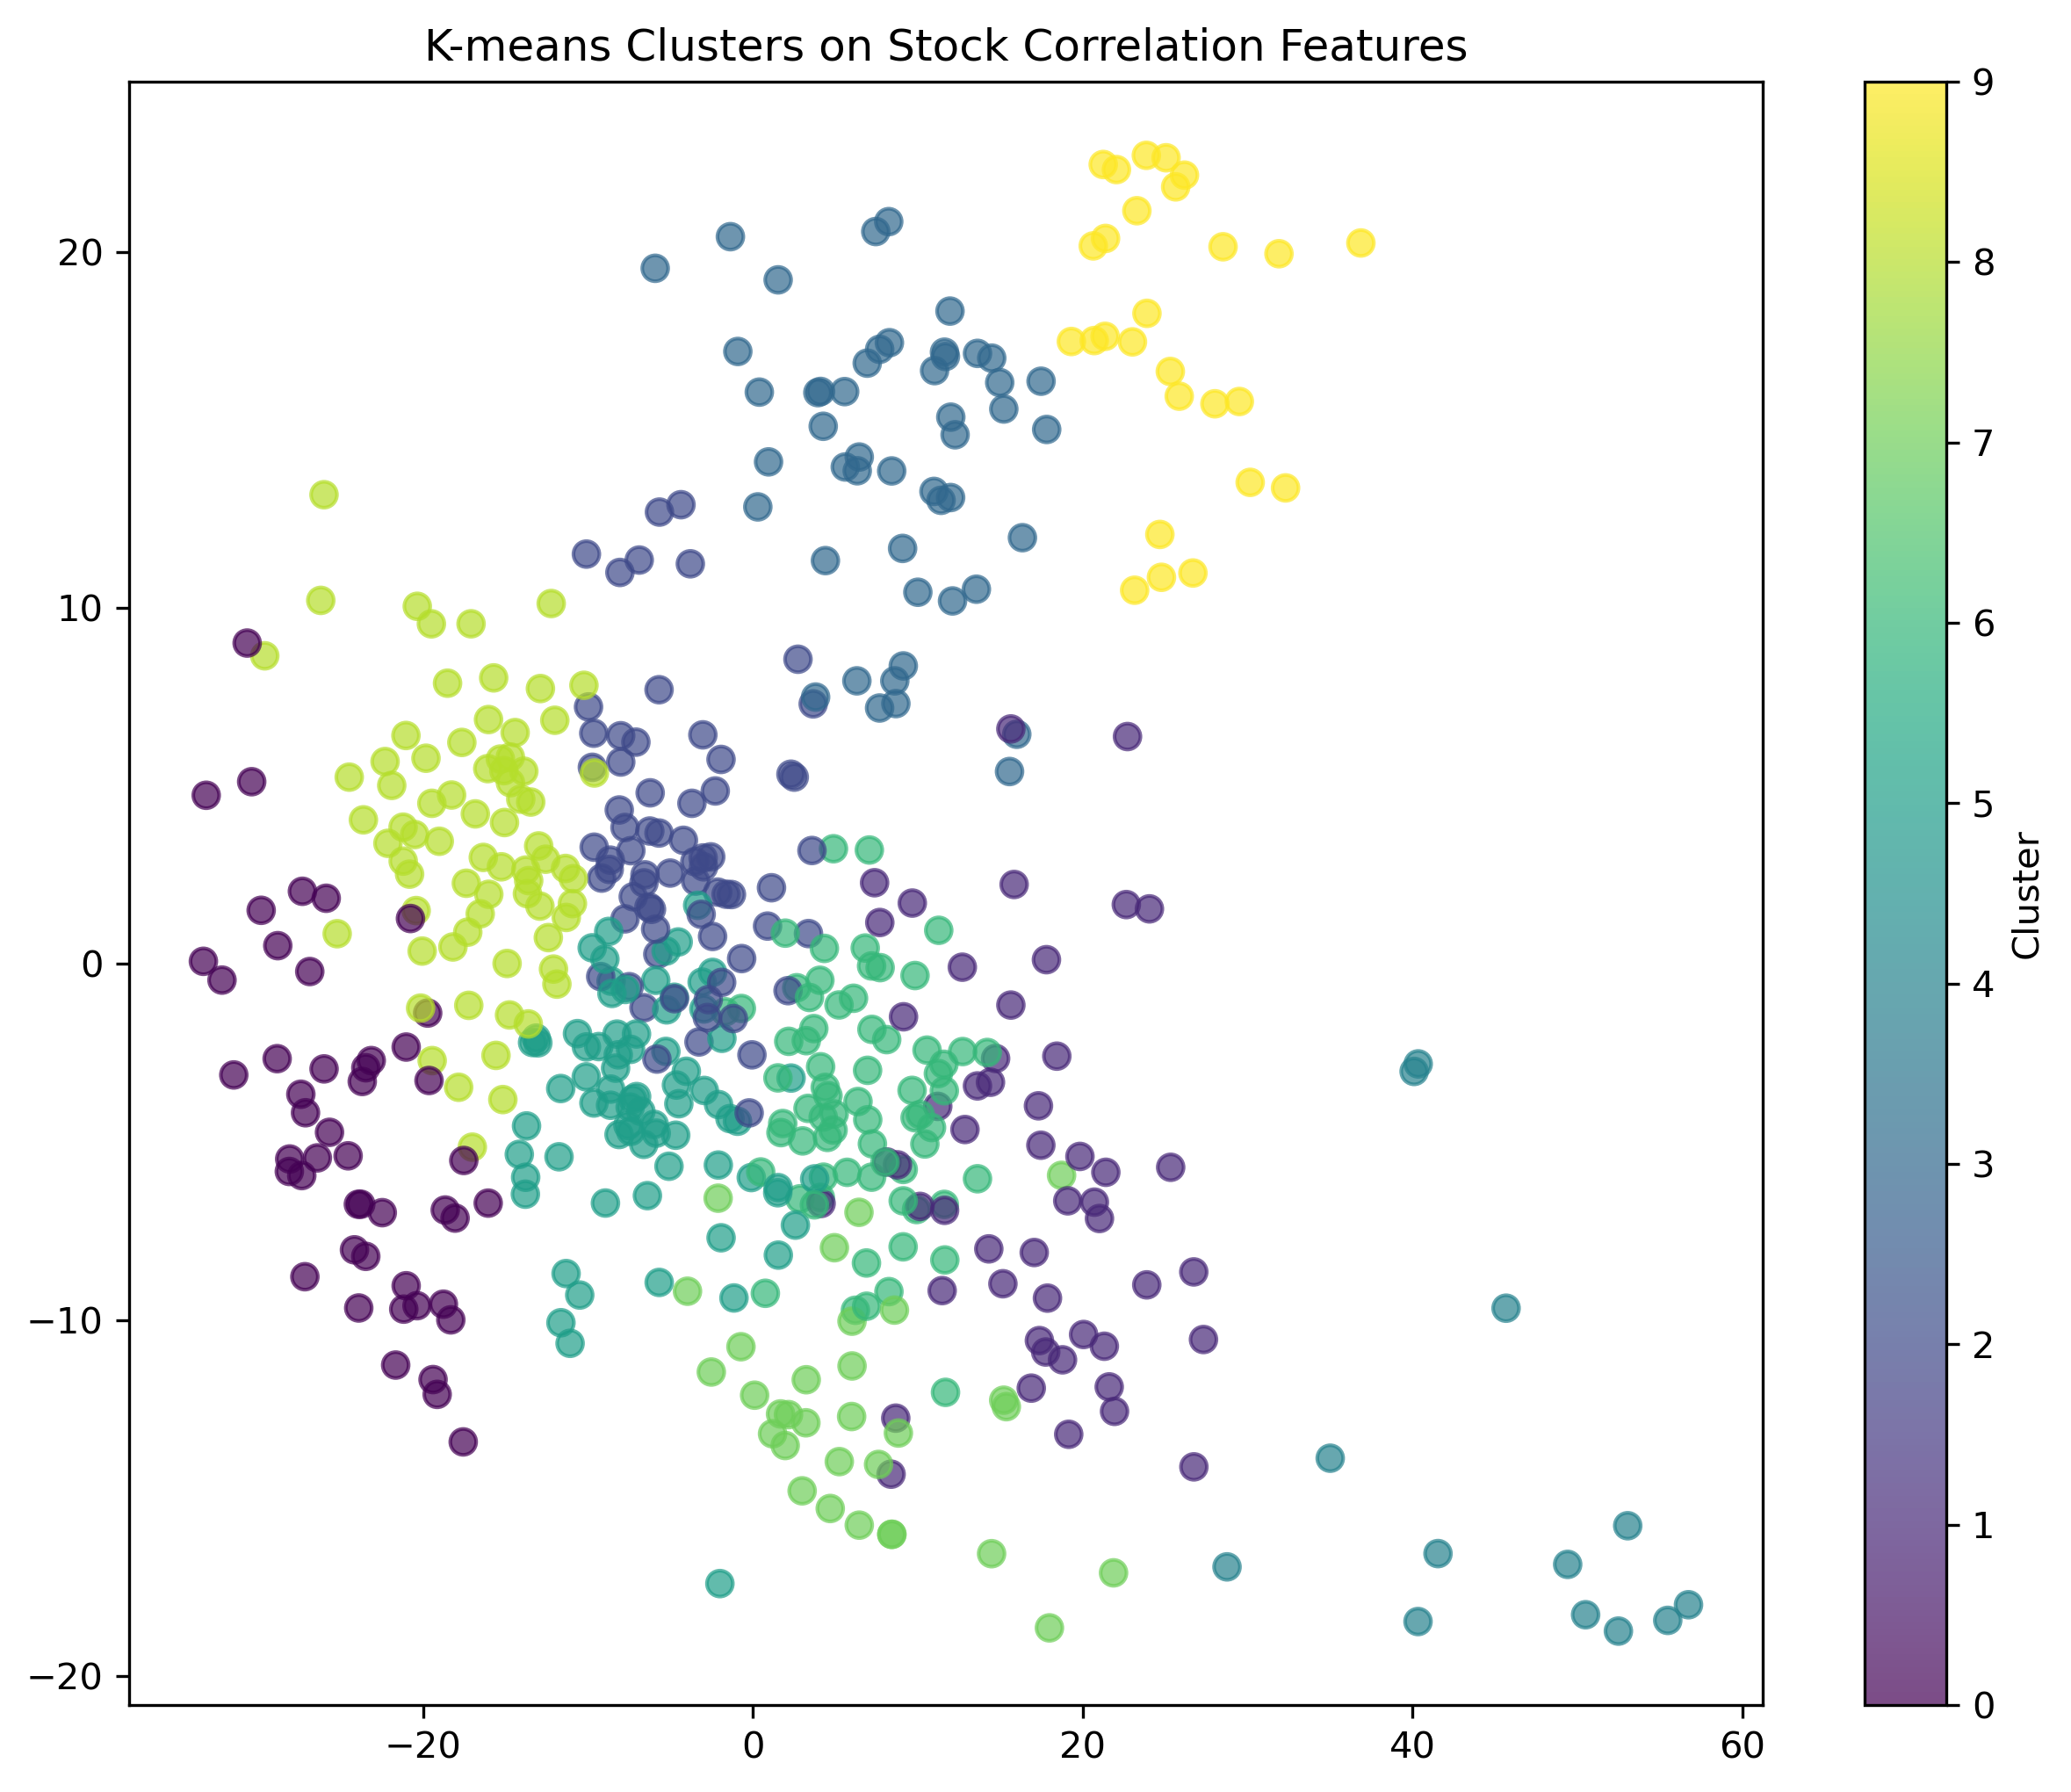
\includegraphics[width=\textwidth]{../results/cluster_analysis/feature_clusters.png}
        \caption{Clusters derived from GNN embeddings (silhouette score: 0.19)}
        \label{fig:feature_clusters}
    \end{minipage}\hfill
    \begin{minipage}{0.48\textwidth}
        \centering
        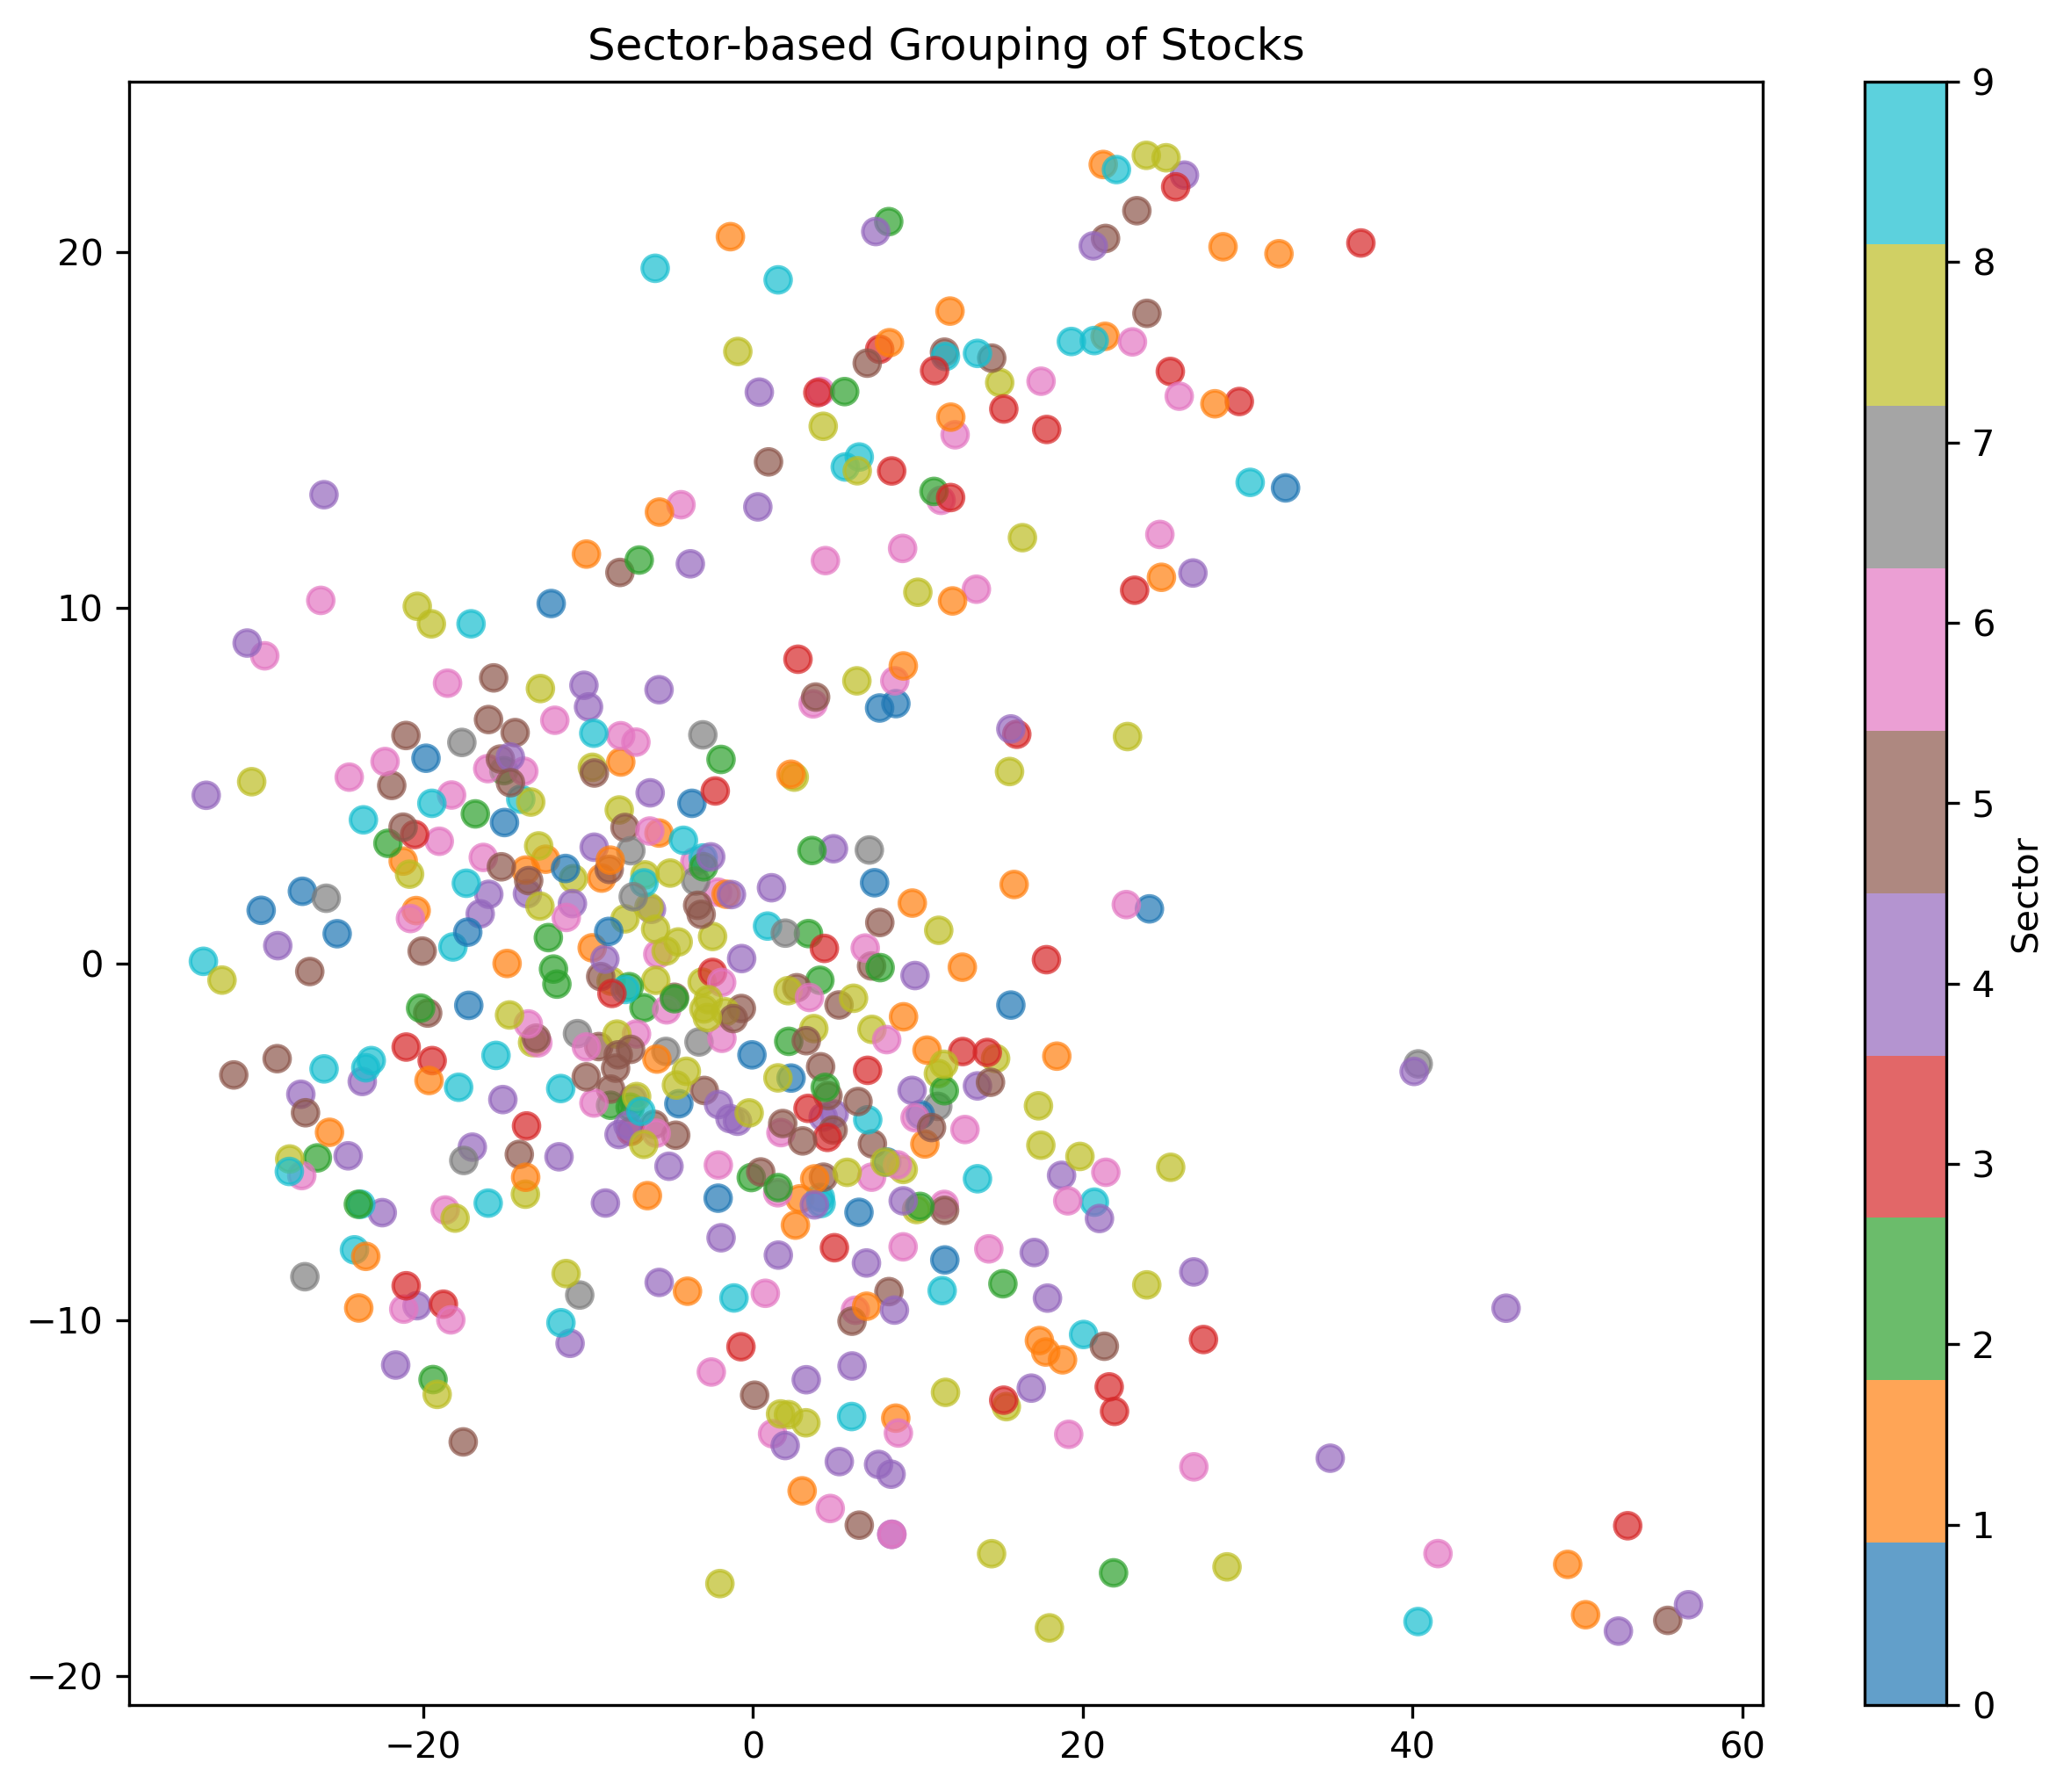
\includegraphics[width=\textwidth]{../results/cluster_analysis/sector_clusters.png}
        \caption{Traditional sector-based clusters (silhouette score: -0.09)}
        \label{fig:sector_clusters}
    \end{minipage}
\end{figure}

The results showed that feature-based clustering using HAD-GNN embeddings produced a silhouette score of approximately 0.19 (Figure \ref{fig:feature_clusters}), significantly outperforming sector-based grouping which had a negative score of -0.09 (Figure \ref{fig:sector_clusters}). This indicates that our model uncovered more coherent stock relationships than those defined by standard industry classifications.

The superior clustering performance suggests that our model identified latent market structures that transcend traditional sector boundaries, potentially capturing more complex financial relationships based on factors such as:

\begin{itemize}
    \item Similar market behavior under specific conditions
    \item Co-movement during market stress periods
    \item Shared exposure to underlying economic factors
\end{itemize}

The visualization in Figure \ref{fig:feature_clusters} reveals more coherent and separated clusters compared to the sector-based groupings in Figure \ref{fig:sector_clusters}, visually confirming the quantitative silhouette score analysis.

\section{Discussion and Conclusion}

Our work demonstrates the value of geometric deep learning approaches for financial market analysis. By progressing from static to dynamic graph models and incorporating hybrid attention mechanisms, we have developed a more nuanced understanding of stock market co-movements that adapts to changing market conditions.

The HAD-GNN approach offers several key insights:

\begin{enumerate}
    \item \textbf{Dynamic Relationships}: Financial networks are inherently temporal, and models that account for this evolution outperform static approaches.
    \item \textbf{Hybrid Attention}: Combining spatial and temporal attention mechanisms allows the model to focus on both important stock relationships and relevant time periods.
    \item \textbf{Latent Structure Discovery}: GNN-based embeddings reveal coherent market structures that are not captured by traditional sector classifications.
\end{enumerate}

\subsection{Limitations and Future Work}

While our model shows promising results, several limitations and directions for future work remain:

\begin{itemize}
    \item \textbf{Graph Construction}: Exploring alternative methods beyond Pearson correlation, such as partial correlation, transfer entropy, or Granger causality
    \item \textbf{Explainability}: Developing techniques to interpret the learned attention weights and node embeddings
    \item \textbf{Multi-resolution Analysis}: Incorporating different time scales to capture both short and long-term dependencies
    \item \textbf{External Information}: Integrating market sentiment, news events, and macroeconomic indicators into the graph structure
\end{itemize}

In conclusion, our HAD-GNN approach demonstrates the potential of geometric deep learning for understanding complex financial systems. By modeling stocks as nodes in a dynamic graph and learning their relationships through hybrid attention mechanisms, we can uncover hidden structures in the market that traditional methods miss. This approach not only improves predictive capabilities but also enhances our understanding of the underlying dynamics driving financial markets.

\bibliographystyle{plain}
\begin{thebibliography}{9}

\bibitem{mantegna1999} 
Mantegna, R. N. (1999). 
\textit{Hierarchical Structure in Financial Markets}. 
The European Physical Journal B, 11(1), 193--197.

\bibitem{kipf2017} 
Kipf, T. N. \& Welling, M. (2017). 
\textit{Semi-Supervised Classification with Graph Convolutional Networks}. 
ICLR 2017.

\bibitem{wu2020} 
Wu, Z. et al. (2020). 
\textit{A Comprehensive Survey on Graph Neural Networks}. 
IEEE Transactions on Neural Networks and Learning Systems.

\bibitem{belkin2003} 
Belkin, M. \& Niyogi, P. (2003). 
\textit{Laplacian Eigenmaps for Dimensionality Reduction and Data Representation}. 
Neural Computation, 15(6), 1373--1396.

\bibitem{velivckovic2018}
Veličković, P., Cucurull, G., Casanova, A., Romero, A., Lio, P., \& Bengio, Y. (2018).
\textit{Graph Attention Networks}.
ICLR 2018.

\bibitem{chen2020}
Chen, S., Poon, K., Soun, J., Topcu, U. (2020).
\textit{Attention-Based Temporal Graph Convolutional Network for Stock Price Prediction}.
ECML-PKDD 2020.

\bibitem{matsunaga2019}
Matsunaga, D., Suzumura, T., & Takahashi, T. (2019).
\textit{Exploring Graph Neural Networks for Stock Market Predictions with Rolling Window Analysis}.
arXiv preprint arXiv:1909.10660.

\end{thebibliography}

\end{document}
